% Template pour faire aide-mémoire
\documentclass[10pt, french]{article}



%% -----------------------------
%% Préambule
%% -----------------------------
% !TEX encoding = UTF-8 Unicode
% LaTeX Preamble for all cheatsheets
% Author : Gabriel Crépeault-Cauchon

% HOW-TO : copy-paste this file in the same directory as your .tex file, and add in your preamble the next command right after you have specified your documentclass : 
% \input{preamble-cheatsht.tex}
% ---------------------------------------------
% ---------------------------------------------

% Extra note : this preamble creates document that are meant to be used inside the multicols environment. See the documentation on internet for further information.

%% -----------------------------
%% Encoding packages
%% -----------------------------
\usepackage[utf8]{inputenc}
\usepackage[T1]{fontenc}
\usepackage{babel}
\usepackage{lmodern}

%% -----------------------------
%% Variable definition
%% -----------------------------
\def\auteur{Gabriel Crépeault-Cauchon / Nicholas Langevin}
\def\BackgroundColor{white}

%% -----------------------------
%% Margin and layout
%% -----------------------------
% Determine the margin for cheatsheet
\usepackage[landscape, hmargin=1cm, vmargin=1.7cm]{geometry}
\usepackage{multicol}

% Remove automatic indentation after section/subsection title.
\setlength{\parindent}{0cm}

% Save space in cheatsheet by removing space between align environment and normal text.
\usepackage{etoolbox}
\newcommand{\zerodisplayskips}{%
  \setlength{\abovedisplayskip}{0pt}%
  \setlength{\belowdisplayskip}{0pt}%
  \setlength{\abovedisplayshortskip}{0pt}%
  \setlength{\belowdisplayshortskip}{0pt}}
\appto{\normalsize}{\zerodisplayskips}
\appto{\small}{\zerodisplayskips}
\appto{\footnotesize}{\zerodisplayskips}

%% -----------------------------
%% URL and links
%% -----------------------------
\usepackage{hyperref}
\hypersetup{colorlinks = true, urlcolor = gray!70!white, linkcolor = black}

%% -----------------------------
%% Document policy (uncomment only one)
%% -----------------------------
%	\usepackage{concrete}
	\usepackage{mathpazo}
%	\usepackage{frcursive} %% permet d'écrire en lettres attachées
%	\usepackage{aeguill}
%	\usepackage{mathptmx}
%	\usepackage{fourier} 

%% -----------------------------
%% Math configuration
%% -----------------------------
\usepackage[fleqn]{amsmath}
\usepackage{amsthm,amssymb,latexsym,amsfonts}
\usepackage{empheq}
\usepackage{numprint}
\usepackage{dsfont} % Pour avoir le symbole du domaine Z

% Mathematics shortcuts

\newcommand{\reels}{\mathbb{R}}
\newcommand{\entiers}{\mathbb{Z}}
\newcommand{\naturels}{\mathbb{N}}
\newcommand{\eval}{\biggr \rvert}
\usepackage{cancel}
\newcommand{\derivee}[1]{\frac{\partial}{\partial #1}}
\newcommand{\prob}[1]{\Pr \left( #1 \right)}
\newcommand{\esp}[1]{\mathrm{E} \left[ #1 \right]} % espérance
\newcommand{\variance}[1]{\mathrm{Var} \left( #1   \right)}
\newcommand{\covar}[1]{\mathrm{Cov} \left( #1   \right)}
\newcommand{\laplace}{\mathcal{L}}
\newcommand{\deriv}[2][]{\frac{\partial^{#1}}{\partial #2^{#1}}}
\newcommand{\e}[1]{\mathrm{e}^{#1}}
\newcommand{\te}[1]{\text{exp}\left\{#1\right\}}
\DeclareMathSymbol{\shortminus}{\mathbin}{AMSa}{"39}



% To indicate equation number on a specific line in align environment
\newcommand\numberthis{\addtocounter{equation}{1}\tag{\theequation}}

%
% Actuarial notation packages
%
\usepackage{actuarialsymbol}
\usepackage{actuarialangle}

%
% Matrix notation for math symbols (\bm{•})
%
\usepackage{bm}
% Matrix notation variable (bold style)
\newcommand{\matr}[1]{\mathbf{#1}}



%% -----------------------------
%% tcolorbox configuration
%% -----------------------------
\usepackage[most]{tcolorbox}
\tcbuselibrary{xparse}
\tcbuselibrary{breakable}

%%
%% Coloured box "definition" for definitions
%%
\DeclareTColorBox{definition}{ o }				% #1 parameter
{
	colframe=blue!60!green,colback=blue!5!white, % color of the box
	breakable, 
	pad at break* = 0mm, 						% to split the box
	title = {#1},
	after title = {\large \hfill \faBook},
}
%%
%% Coloured box "definition2" for definitions
%%
\DeclareTColorBox{definitionNOHFILL}{ o }				% #1 parameter
{
	colframe=blue!60!green,colback=blue!5!white, % color of the box
	pad at break* = 0mm, 						% to split the box
	title = {#1},
	before title = {\faBook \quad },
	breakable
}


%%
%% Coloured box "algo" for algorithms
%%
\newtcolorbox{algo}[ 1 ]
{
	colback = blue!5!white,
	colframe = blue!75!black,
	title=#1,
	fonttitle = \bfseries,
	breakable
}
%%
%% Coloured box "conceptgen" for points adding to a concept's deifintion
%%
\newtcolorbox{conceptgen}[ 1 ]
{
	breakable,
	colback = beaublue,
	colframe = airforceblue,
	title=#1,
	fonttitle = \bfseries
}
%%
%% Coloured box "probch3" pour formules relatives au 3ème chapitre de prob
%%
\newtcolorbox{probch3}[ 1 ]
{
	colback = ruddypink,
	colframe = burgundy,
	fonttitle = \bfseries,	
	breakable,
	title=#1
}
%%
%% Coloured box "formula" for formulas
%%
\newtcolorbox{formula}[ 1 ]
{
	colback = green!5!white,
	colframe = green!70!black,
	breakable,
	fonttitle = \bfseries,
	title=#1
}
%%
%% Coloured box "formula" for formulas
%%
\DeclareTColorBox{algo2}{ o }
{
	enhanced,
	title = #1,
	colback=blue!5!white,	
	colbacktitle=blue!75!black,
	fonttitle = \bfseries,
	breakable,
	boxed title style={size=small,colframe=arsenic} ,
	attach boxed title to top center = {yshift=-3mm,yshifttext=-1mm},
}
%%
%% Coloured box "examplebox" for formulas
%%
\newtcolorbox{examplebox}[ 1 ]
{
	colback = lightmauve,
	colframe = antiquefuchsia,
	breakable,
	fonttitle = \bfseries,title=#1
}
%%
%% Coloured box "rappel" pour rappel de formules
%%
\newtcolorbox{rappel}[ 1 ]
{
	colback = ashgrey,
	colframe = arsenic,
	breakable,
	fonttitle = \bfseries,title=#1
}
%%
%% Coloured box "rappel" pour rappel de formules
%%
\DeclareTColorBox{rappel_enhanced}{ o }
{
	enhanced,
	title = #1,
	colback=ashgrey, % color of the box
%	colframe=blue(pigment),
%	colframe=arsenic,	
	colbacktitle=arsenic,
	fonttitle = \bfseries,
	breakable,
	boxed title style={size=small,colframe=arsenic} ,
	attach boxed title to top center = {yshift=-3mm,yshifttext=-1mm},
}
%%
%% Coloured box "notation" for notation and terminology
%%
\DeclareTColorBox{distributions}{ o }			% #1 parameter
{
	enhanced,
	title = #1,
	colback=gray(x11gray), % color of the box
%	colframe=blue(pigment),
	colframe=arsenic,	
	colbacktitle=aurometalsaurus,
	fonttitle = \bfseries,
	boxed title style={size=small,colframe=arsenic} ,
	attach boxed title to top center = {yshift=-3mm,yshifttext=-1mm},
	breakable
%	left=0pt,
%  	right=0pt,
%    box align=center,
%    ams align*
%  	top=-10pt
}

%% -----------------------------
%% Graphics and pictures
%% -----------------------------
\usepackage{graphicx}
\usepackage{pict2e}
\usepackage{tikz}

%% -----------------------------
%% insert pdf pages into document
%% -----------------------------
\usepackage{pdfpages}

%% -----------------------------
%% Color configuration
%% -----------------------------
\usepackage{color, soulutf8, colortbl}


%
%	Colour definitions
%
\definecolor{blue(munsell)}{rgb}{0.0, 0.5, 0.69}
\definecolor{blue(matcha)}{rgb}{0.596, 0.819, 1.00}
\definecolor{blue(munsell)-light}{rgb}{0.5, 0.8, 0.9}
\definecolor{bleudefrance}{rgb}{0.19, 0.55, 0.91}
\definecolor{blizzardblue}{rgb}{0.67, 0.9, 0.93}
\definecolor{bondiblue}{rgb}{0.0, 0.58, 0.71}
\definecolor{blue(pigment)}{rgb}{0.2, 0.2, 0.6}
\definecolor{bluebell}{rgb}{0.64, 0.64, 0.82}
\definecolor{airforceblue}{rgb}{0.36, 0.54, 0.66}
\definecolor{beaublue}{rgb}{0.74, 0.83, 0.9}
\definecolor{cobalt}{rgb}{0.0, 0.28, 0.67}	% nice light blue-ish
\definecolor{blue_rectangle}{RGB}{83, 84, 244}		% ACT-2004
\definecolor{indigo(web)}{rgb}{0.29, 0.0, 0.51}	% purple-ish
\definecolor{antiquefuchsia}{rgb}{0.57, 0.36, 0.51}	%	pastel dark purple ish
\definecolor{darkpastelpurple}{rgb}{0.59, 0.44, 0.84}
\definecolor{gray(x11gray)}{rgb}{0.75, 0.75, 0.75}
\definecolor{aurometalsaurus}{rgb}{0.43, 0.5, 0.5}
\definecolor{ruddypink}{rgb}{0.88, 0.56, 0.59}
\definecolor{pastelred}{rgb}{1.0, 0.41, 0.38}		
\definecolor{lightmauve}{rgb}{0.86, 0.82, 1.0}
\definecolor{azure(colorwheel)}{rgb}{0.0, 0.5, 1.0}
\definecolor{darkgreen}{rgb}{0.0, 0.2, 0.13}			
\definecolor{burntorange}{rgb}{0.8, 0.33, 0.0}		
\definecolor{burntsienna}{rgb}{0.91, 0.45, 0.32}		
\definecolor{ao(english)}{rgb}{0.0, 0.5, 0.0}		% ACT-2003
\definecolor{amber(sae/ece)}{rgb}{1.0, 0.49, 0.0} 	% ACT-2004
\definecolor{green_rectangle}{RGB}{131, 176, 84}		% ACT-2004
\definecolor{red_rectangle}{RGB}{241,112,113}		% ACT-2004
\definecolor{amethyst}{rgb}{0.6, 0.4, 0.8}
\definecolor{amethyst-light}{rgb}{0.6, 0.4, 0.8}
\definecolor{ashgrey}{rgb}{0.7, 0.75, 0.71}			% dark grey-black-ish
\definecolor{arsenic}{rgb}{0.23, 0.27, 0.29}			% light green-beige-ish gray
\definecolor{amaranth}{rgb}{0.9, 0.17, 0.31}
\definecolor{brickred}{rgb}{0.8, 0.25, 0.33}
\definecolor{pastelred}{rgb}{1.0, 0.41, 0.38}

%
% Useful shortcuts for coloured text
%
\newcommand{\orange}{\textcolor{orange}}
\newcommand{\red}{\textcolor{red}}
\newcommand{\cyan}{\textcolor{cyan}}
\newcommand{\blue}{\textcolor{blue}}
\newcommand{\green}{\textcolor{green}}
\newcommand{\purple}{\textcolor{magenta}}
\newcommand{\yellow}{\textcolor{yellow}}

%% -----------------------------
%% Enumerate environment configuration
%% -----------------------------
%
% Custum enumerate & itemize Package
%
\usepackage{enumitem}
%
% French Setup for itemize function
%
\frenchbsetup{StandardItemLabels=true}
%
% Change default label for itemize
%
\renewcommand{\labelitemi}{\faAngleRight}


%% -----------------------------
%% Tabular column type configuration
%% -----------------------------
\newcolumntype{C}{>{$}c<{$}} % math-mode version of "l" column type
\newcolumntype{L}{>{$}l<{$}} % math-mode version of "l" column type
\newcolumntype{R}{>{$}r<{$}} % math-mode version of "l" column type
\newcolumntype{f}{>{\columncolor{green!20!white}}p{1cm}}
\newcolumntype{g}{>{\columncolor{green!40!white}}m{1.2cm}}
\newcolumntype{a}{>{\columncolor{red!20!white}$}p{2cm}<{$}}	% ACT-2005
% configuration to force a line break within a single cell
\usepackage{makecell}


%% -----------------------------
%% Fontawesome for special symbols
%% -----------------------------
\usepackage{fontawesome}

%% -----------------------------
%% Section Font customization
%% -----------------------------
\usepackage{sectsty}
\sectionfont{\color{\SectionColor}}
\subsectionfont{\color{\SubSectionColor}}

%% -----------------------------
%% Footer/Header Customization
%% -----------------------------
\usepackage{lastpage}
\usepackage{fancyhdr}
\pagestyle{fancy}

%
% Header
%
\fancyhead{} 	% Reset
\fancyhead[L]{Aide-mémoire pour~ \cours ~(\textbf{\sigle})}
\fancyhead[R]{\auteur}

%
% Footer
%
\fancyfoot{}		% Reset
\fancyfoot[R]{\thepage ~de~ \pageref{LastPage}}
\fancyfoot[L]{\href{https://github.com/ressources-act/Guide_de_survie_en_actuariat}{\faGithub \ ressources-act/Guide de survie en actuariat}}
%
% Page background color
%
\pagecolor{\BackgroundColor}




%% END OF PREAMBLE
% ---------------------------------------------
% ---------------------------------------------
%% -----------------------------
%% Variable definition
%% -----------------------------
\def\cours{Mathématiques Financières}
\def\sigle{ACT-1001}
%% -----------------------------
%% Colour setup for sections
%% -----------------------------
\def\SectionColor{burntorange}
\def\SubSectionColor{burntsienna}
\def\SubSubSectionColor{burntsienna}
%% -----------------------------
%% Colour setup for prestations
%%	Ajoute couleurs sur les trêmas des signes de prestations
%% -----------------------------
\usepackage{stackengine}
\newcommand\cumlaut[2][black]{\stackon[.33ex]{#2}{\textcolor{#1}{\kern-.04ex.\kern-.2ex.}}}
%
% Save more space than default
%
\setlength{\abovedisplayskip}{-15pt}
\setlist{leftmargin=*}
%
%	Extra math symbols
%
\usepackage{mathrsfs}
\usetikzlibrary{matrix}
%
% thin space, limits underneath in displays
%

%% -----------------------------
%% 	Colour setup for sections
%% -----------------------------
\def\SectionColor{cobalt}
\def\SubSectionColor{azure(colorwheel)}
\def\SubSubSection{azure(colorwheel)}
%% -----------------------------
\setcounter{secnumdepth}{0}

%% -----------------------------
%% Color definitions
%% -----------------------------
\definecolor{indigo(web)}{rgb}{0.29, 0.0, 0.51}
\definecolor{cobalt}{rgb}{0.0, 0.28, 0.67}
\definecolor{azure(colorwheel)}{rgb}{0.0, 0.5, 1.0}
%% -----------------------------
%% Variable definition
%% -----------------------------
%%
%% Matrix notation variable (bold style)
%%
\newcommand\cololine[2]{\colorlet{temp}{.}\color{#1}\bar{\color{temp}#2}\color{temp}}
\newcommand\colbar[2]{\colorlet{temp}{.}\color{#1}\bar{\color{temp}#2}\color{temp}}

\begin{document}

\begin{center}
	\textsc{\Large Contributeurs}\\[0.5cm] 
\end{center}
\begin{contrib}{ACT-1XXX\: Cours de première année}
\begin{description}
	\item[aut., cre.] Alec James van Rassel
\end{description}
\end{contrib}

\newpage
\raggedcolumns
\begin{multicols*}{2}

\section{Compléments de mathématiques}
\subsection*{Algèbre linéaire}
Soit :
\begin{align*}
	\frac{A}{B}	
	&=	Q \text{ remainder } R
\end{align*}
où 
\begin{description}
	\item[$A$]	Nombre dividende.
	\item[$B$]	Nombre diviseur.
		\begin{itemize}
		\item	Selon la deuxième équation ci-dessous, on l'appel le \textit{module}.
		\end{itemize}
	\item[$Q$]	Quotient.
	\item[$R$]	Restant.
\end{description}

On peut donc aussi trouver que \lfbox[formula]{$A \mod B = R$}.

L'opérateur de congruence $\equiv$ nous indique que 2 nombres ont le même restant.
Donc, $A \equiv B (\mod C)$ implique que $A \mod C = B \mod C$.
\begin{itemize}
	\item P. ex., $26 \mod 5	=	1$ et $11 \mod 5 = 1$ donc $26 \equiv 11 (\mod 5)$.
\end{itemize}

\subsection*{Intégrales utiles à connaître}
\begin{conceptgen}{Polynômes}
\begin{align*}
	\int \frac{1}{ax + b} dx 
	&=	\frac{1}{a} \ln(ax + b) + C	&
	\int x^{\frac{p}{q}}dx
	&=	\frac{q}{p + q} x^{\frac{p + q}{q}} + C	
\end{align*}
\end{conceptgen}

\begin{conceptgen}{Fonctions exponentielles et logarithmiques}
\begin{align*}
	\int a^{x} dx 
	&=	\frac{a^{x}}{\ln(a)} + C	&
	\int \ln(x) dx 
	&=	x \ln(x) - x + C	
\end{align*}
\end{conceptgen}

\subsection*{Dérivées utiles à connaître}

\begin{align*}
	\derivee{x}(a^{x})
	&=	a^{x}\ln(a)	\\
	\derivee{x}(\sin(x))
	&=	\cos(x)	&
	\derivee{x}(\cos(x))
	&=	-\sin(x)	\\	
\end{align*}

\subsection*{Aires de formes}

\begin{center}
\tikzset{every picture/.style={line width=0.75pt}} %set default line width to 0.75pt        

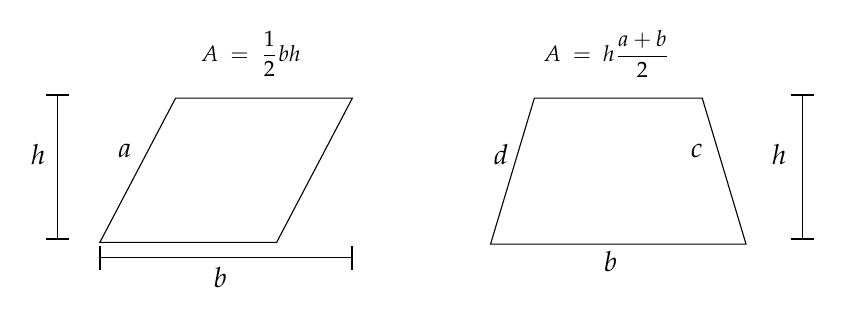
\begin{tikzpicture}[x=0.75pt,y=0.75pt,yscale=-1,xscale=1]
%uncomment if require: \path (0,300); %set diagram left start at 0, and has height of 300

%Shape: Parallelogram [id:dp190851926021818] 
\draw   (123,67.67) -- (208.17,67.67) -- (171.67,137.19) -- (86.5,137.19) -- cycle ;
%Straight Lines [id:da028760448720356768] 
\draw    (66,66.33) -- (66,135.67) ;
\draw [shift={(66,135.67)}, rotate = 270] [color={rgb, 255:red, 0; green, 0; blue, 0 }  ][line width=0.75]    (0,5.59) -- (0,-5.59)   ;
\draw [shift={(66,66.33)}, rotate = 270] [color={rgb, 255:red, 0; green, 0; blue, 0 }  ][line width=0.75]    (0,5.59) -- (0,-5.59)   ;
%Straight Lines [id:da16729889993203217] 
\draw    (86.5,144.67) -- (208.17,144.67) ;
\draw [shift={(208.17,144.67)}, rotate = 180] [color={rgb, 255:red, 0; green, 0; blue, 0 }  ][line width=0.75]    (0,5.59) -- (0,-5.59)   ;
\draw [shift={(86.5,144.67)}, rotate = 180] [color={rgb, 255:red, 0; green, 0; blue, 0 }  ][line width=0.75]    (0,5.59) -- (0,-5.59)   ;
%Straight Lines [id:da8024064344696678] 
\draw    (425,66.33) -- (425,135.67) ;
\draw [shift={(425,135.67)}, rotate = 270] [color={rgb, 255:red, 0; green, 0; blue, 0 }  ][line width=0.75]    (0,5.59) -- (0,-5.59)   ;
\draw [shift={(425,66.33)}, rotate = 270] [color={rgb, 255:red, 0; green, 0; blue, 0 }  ][line width=0.75]    (0,5.59) -- (0,-5.59)   ;
%Shape: Trapezoid [id:dp7515796089887394] 
\draw   (274.75,138) -- (295.85,67.67) -- (376.73,67.67) -- (397.83,138) -- cycle ;

% Text Node
\draw (140,148) node [anchor=north west][inner sep=0.75pt]   [align=left] {$\displaystyle b$};
% Text Node
\draw (52,88.5) node [anchor=north west][inner sep=0.75pt]   [align=left] {$\displaystyle h$};
% Text Node
\draw (94,88.5) node [anchor=north west][inner sep=0.75pt]   [align=left] {$\displaystyle a$};
% Text Node
\draw (134,34) node [anchor=north west][inner sep=0.75pt]  [font=\footnotesize] [align=left] {$\displaystyle A\ =\ \frac{1}{2} bh$};
% Text Node
\draw (328,140) node [anchor=north west][inner sep=0.75pt]   [align=left] {$\displaystyle b$};
% Text Node
\draw (409,88.5) node [anchor=north west][inner sep=0.75pt]   [align=left] {$\displaystyle h$};
% Text Node
\draw (275,88.5) node [anchor=north west][inner sep=0.75pt]   [align=left] {$\displaystyle d$};
% Text Node
\draw (299,34) node [anchor=north west][inner sep=0.75pt]  [font=\footnotesize] [align=left] {$\displaystyle A\ =\ h\frac{a+b}{2}$};
% Text Node
\draw (370,88.5) node [anchor=north west][inner sep=0.75pt]   [align=left] {$\displaystyle c$};


\end{tikzpicture}
\end{center}

\subsection*{Moyennes}
La moyenne de $n$ chiffres $x_{1}, x_{2}, \dots, x_{n}$.

\begin{rappel_enhanced}[Moyenne arithmétique]
\begin{align*}
	A(x)
	&=	\frac{1}{n}\sumz{n}{i = 1} x_{i}
	=	\frac{x_{1} + x_{2} + \hdots + x_{n}}{n}
\end{align*}
\end{rappel_enhanced}

\begin{rappel_enhanced}[Moyenne géométrique]
\begin{align*}
	G(x)
	&=	\left(\prod^{n}_{i = 1} x_{i}\right)^{1/n}
	=	\left(x_{1} \times x_{2} \times \hdots \times x_{n}\right)^{1/n}
\end{align*}
\end{rappel_enhanced}

\paragraph{Note:}	\icbox[red][palechestnut]{$G(x)	\leq		A(x)$}.

\subsection*{Sommations}
\begin{align*}
\sum_{k = m}^{n} r^k &= r^{m} \frac{1 - r^{n - m + 1}}{1 - r} &
\sum_{k = 0}^{\infty}k v^k &= \frac{v}{(1 - v)^2} \\
\sum_{k = 1}^{n}k^{\textcolor{teal}{3}} &= \textcolor{teal}{\bigg(}\frac{n(n + 1)}{2}\textcolor{teal}{\bigg)^{2}} &
\sum_{k = 1}^{n}k^2 &= \frac{n(n + 1)(2n + 1)}{6} \\
\end{align*}

\subsection{Différenciation}
\begin{rappel_enhanced}[Théorème des accroissements finis]
\begin{rappel_enhanced}[Théorème de Rolle]
Soit la fonction $f$ qui répond aux critères suivants :
\begin{enumerate}
	\item	$f(x)$ est continue sur l'intervalle fermé $[a, b]$ ;
	\item	$f(x)$ est différentiable sur l'intervalle ouvert $(a, b)$ ;
	\item	$f(a)	=	f(b)$.
\end{enumerate}
Alors, il existe un nombre $c$ tel que \lfbox[conditions]{$a < c < b$} et \lfbox[formula]{$f'(c)	= 0$}; c'est-à-dire, $f(x)$ a un point critique dans $(a, b)$.
\end{rappel_enhanced}

Soit la fonction $f$ qui répond aux critères suivants :
\begin{enumerate}
	\item	$f(x)$ est continue sur l'intervalle fermé $[a, b]$ ;
	\item	$f(x)$ est différentiable sur l'intervalle ouvert $(a, b)$.
\end{enumerate}
Alors, il existe un nombre $c$ tel que \lfbox[conditions]{$a < c < b$} et \lfbox[formula]{$f'(c)	=	\frac{f(b) - f(a)}{b - a}$}.
\end{rappel_enhanced}


\subsection*{Estimation Taylor}
\begin{align*}
	f(x) 
		&=	\sum_{n = 0}^{\infty} \frac{f^{(n)}(x_0)}{n!}(x - x_0)^{n} \\
		&\approx f(x_0) + f'(x_0) (x - x_0)
\end{align*}

\begin{definitionNOHFILL}[Théorème de Leibnitz]
Soit: 
\begin{itemize}
	\item 	une fonction $f(x, \alpha)$ continue sur $[a, b]$ et
	\item des fonctions (dérivables) de $\alpha$, $u(\alpha)$ et $v(\alpha)$, prenant valeur dans $[a, b]$.
\end{itemize}
Alors,

	\setlength{\mathindent}{-.24cm}
\begin{equation*}
	\deriv{\alpha}{} \int_{u(\alpha)}^{v(\alpha)} f(x, \alpha) dx = 
	\int_{u(\alpha)}^{v(\alpha)} \deriv{\alpha}{}  f(x, \alpha) dx + f(v(\alpha), \alpha) \deriv{\alpha}{} v(\alpha) - f(u(\alpha), \alpha) \deriv{\alpha}{} u(\alpha)
\end{equation*}
	\setlength{\mathindent}{1cm}
\end{definitionNOHFILL}

\begin{definitionNOHFILL}[Domaines]
\begin{description}
	\item[$\mathds{R}$]: Real numbers, $x \in (-\infty, \infty)$.
	\item[$\mathds{Z}$]: Integers; all integers positive \& negative, $x \in \{\dots, -3, -2, -1, 0, 1, 2, 3, \dots\}$.
	\item[$\mathds{N}$]: Natural numbers; all positive integers numbers, $x \in \{1, 2, 3, \dots\}$.
	\item[$\mathds{Q}$]: Rational numbers; numbers written as fractions, for example $1.25\%$, $-0.4775$, $3.\overline{153}$, $\frac{1}{2}, \frac{4}{7}$.	
	\item[$\mathds{R} \backslash \mathds{Q}$]: Irrational numbers; for example $\pi, \mathrm{e}, \sqrt{3}$.
\end{description}
\end{definitionNOHFILL}

\subsection*{Intégrale de Riemann-Stieltjes}
\begin{rappel_enhanced}[Intégrale de Riemann]
Soit la fonction $f$ continue sur l'intervalle $[a, b]$.
\begin{itemize}
	\item	On divise l'ensemble $[a, b]$ en $n$ sous-intervalles $c_{i} = [x_{i - 1}, x_{i}]$.
	\item	Les $n$ partitions $P$ des sous-intervalles sont aux points $P	=	\{a	=	x_{0} < x_{1} < \hdots < x_{n} = b\}$. 
	\item	La norme des partitions est la longueur du plus long sous-intervalle $\lVert P \rVert	=	\underset{1 \leq i \leq n}{\max}\{|x_{i} - x_{i - 1}|\}$.
	\item	On dénote le $i^{\text{e}}$ point du sous-intervalle $c_{i}$ par $t_{i} \in [x_{i - 1}, x_{i}]$.
\end{itemize}

Visuellement :
\begin{center}

\tikzset{every picture/.style={line width=0.75pt}} %set default line width to 0.75pt        

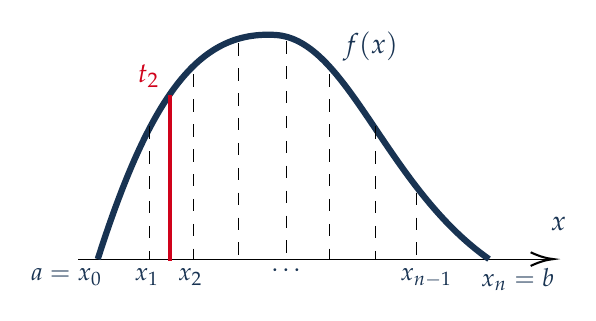
\begin{tikzpicture}[x=0.75pt,y=0.75pt,yscale=-1,xscale=1]
%uncomment if require: \path (0,300); %set diagram left start at 0, and has height of 300

%Straight Lines [id:da21404446917902464] 
\draw    (90.5,170) -- (317.5,170) ;
\draw [shift={(319.5,170)}, rotate = 180] [color={rgb, 255:red, 0; green, 0; blue, 0 }  ][line width=0.75]    (10.93,-3.29) .. controls (6.95,-1.4) and (3.31,-0.3) .. (0,0) .. controls (3.31,0.3) and (6.95,1.4) .. (10.93,3.29)   ;
%Curve Lines [id:da28387606314411706] 
\draw [color={rgb, 255:red, 24; green, 51; blue, 82 }  ,draw opacity=1 ][line width=2.25]    (100,170) .. controls (126.5,87) and (150.5,60) .. (185.5,62) .. controls (220.5,64) and (238.5,135) .. (288.5,170) ;
%Straight Lines [id:da40818193657573865] 
\draw  [dash pattern={on 4.5pt off 4.5pt}]  (125,106) -- (125,170) ;
%Straight Lines [id:da26577873998854695] 
\draw  [dash pattern={on 4.5pt off 4.5pt}]  (146,81) -- (146,170) ;
%Straight Lines [id:da3961268279871215] 
\draw  [dash pattern={on 4.5pt off 4.5pt}]  (168,66) -- (168,173) ;
%Straight Lines [id:da08779208875720568] 
\draw  [dash pattern={on 4.5pt off 4.5pt}]  (191,65) -- (191,172) ;
%Straight Lines [id:da7201407531686637] 
\draw  [dash pattern={on 4.5pt off 4.5pt}]  (211.75,81) -- (211.75,170) ;
%Straight Lines [id:da14334729073326669] 
\draw  [dash pattern={on 4.5pt off 4.5pt}]  (233.75,106) -- (233.75,170) ;
%Straight Lines [id:da5334510980168155] 
\draw  [dash pattern={on 4.5pt off 4.5pt}]  (253.75,138) -- (253.75,173) ;
%Straight Lines [id:da4523334823717404] 
\draw [color={rgb, 255:red, 208; green, 2; blue, 27 }  ,draw opacity=1 ][line width=1.5]    (135,91) -- (135,171) ;

% Text Node
\draw (217,59.4) node [anchor=north west][inner sep=0.75pt]  [color={rgb, 255:red, 24; green, 51; blue, 82 }  ,opacity=1 ]  {$f( x)$};
% Text Node
\draw (317,148.4) node [anchor=north west][inner sep=0.75pt]  [color={rgb, 255:red, 24; green, 51; blue, 82 }  ,opacity=1 ]  {$x$};
% Text Node
\draw (66.5,173.4) node [anchor=north west][inner sep=0.75pt]  [font=\small,color={rgb, 255:red, 24; green, 51; blue, 82 }  ,opacity=1 ]  {$a=x_{0}$};
% Text Node
\draw (116.5,173.4) node [anchor=north west][inner sep=0.75pt]  [font=\small,color={rgb, 255:red, 24; green, 51; blue, 82 }  ,opacity=1 ]  {$x_{1}$};
% Text Node
\draw (137.5,173.4) node [anchor=north west][inner sep=0.75pt]  [font=\small,color={rgb, 255:red, 24; green, 51; blue, 82 }  ,opacity=1 ]  {$x_{2}$};
% Text Node
\draw (244.5,173.4) node [anchor=north west][inner sep=0.75pt]  [font=\small,color={rgb, 255:red, 24; green, 51; blue, 82 }  ,opacity=1 ]  {$x_{n-1}$};
% Text Node
\draw (283.5,173.4) node [anchor=north west][inner sep=0.75pt]  [font=\small,color={rgb, 255:red, 24; green, 51; blue, 82 }  ,opacity=1 ]  {$x_{n} =b$};
% Text Node
\draw (182.5,173.4) node [anchor=north west][inner sep=0.75pt]  [font=\small,color={rgb, 255:red, 24; green, 51; blue, 82 }  ,opacity=1 ]  {$\dotsc $};
% Text Node
\draw (118,75) node [anchor=north west][inner sep=0.75pt]  [color={rgb, 255:red, 208; green, 2; blue, 27 }  ,opacity=1 ] [align=left] {$\displaystyle t_{2}$};
\end{tikzpicture}
\end{center}

On obtient donc l'intégrale de Riemann : \lfbox[formula]{$\limz{\lVert P \rVert}{0}\ \sumz{n}{i = 1} f(t_{i})(x_{i} - x_{i - 1})	=	\int_{a}^{b}f(x)dx$}.
\end{rappel_enhanced}

\begin{rappel_enhanced}[Intégrale de Riemann-\textit{Stieltjes}]
L'intégrale de Riemann-\textit{Stieltjes} généralise l'intégrale de Riemann avec une fonction $g$ comme mesure de distance entre les points $x_{i - 1}$ et $x_{i}$.

\tcbline

Soit les fonction $f, g : [a, b] \rightarrow \mathbb{R}$.\\
On maintient les définitions de l'intégrale de Riemann et substitue $(x_{i - 1} - x_{i})$ pour $\left(g(x_{i - 1}) - g(x_{i})\right)$ pour obtenir l'intégrale de Riemann-Stieltjes : \lfbox[formula]{$\limz{\lVert P \rVert}{0}\ \sumz{n}{i = 1} f(t_{i})(g(x_{i - 1}) - g(x_{i}))	=	\int_{a}^{b}f(x)dg(x)$}.
\end{rappel_enhanced}


\subsection*{Fonction impaire}

Une fonction est impaire \textit{(odd)} lorsque $f(-x) = -f(x)$.\\
Par exemple, $\sin(-x) = -\sin(x)$.

\newpage

\section{Mathématiques financières}

\subsection*{Intérêt simple}
\begin{align*}
	a(t)
		&=	1 + it &
	v(t)
		&=	\frac{1}{1 + it} \\
	\text{Prix}
		&=	100 \left( 1 - \frac{it}{365} \right)^{-1}
\end{align*}

\subsection*{facteurs d'actualisation et d'accumulation}
% [t] tells LaTex to place minipage at the top of the page
\begin{minipage}[t]{.5\linewidth}
\begin{align*}
	a(t) 
		&= 	(1 + i)^{t} 		\\
		&= 	(1 - d)^{-t}	\\
		&= 	e^{\int_{0}^{t} \delta_s ds} 
\end{align*}
\end{minipage}
\begin{minipage}[t]{.5\linewidth}
	\begin{align*}
	v(t) 
		&=	(1 + i)^{-t}		\\
		&=	(1 - d)^{t}	 	\\
		&= 	e^{-\int_{0}^{t} \delta_s ds} 
\end{align*}
\end{minipage}

\subsection*{Conversion de taux}
\begin{align*}
%	i 	&= \left( 1 + \frac{i^{(m)}}{m} \right)^{m} - 1 &
	d	&= 	\frac{i}{1 + i} &
	i^{\mathrm{R}}
		&=	\frac{i - r}{1 + r}
\end{align*}

%\subsection*{Conversion de taux}
\begin{align*}
&\text{Taux d'intérêt \underline{effectif} \textit{annuel}} & 
	& i = \left( 1 + \frac{i^{(m)}}{m} \right)^{m} - 1 \\
&\text{Taux d'intérêt \underline{nominal} \textit{annuel}} & 
	& i^{(m)} = m \left( (1 + i)^{1/m} - 1 \right)	\\
&\text{Taux d'escompte \underline{nominal} \textit{annuel}} & 
	& d^{(m)} = m \left( 1 - (1 - d)^{1/m} \right)
\end{align*}

\subsection*{Rentes constantes}

\begin{align*}
	\cumlaut[cyan]{a}_{\angl{n}}^{\textcolor{red}{(m)}} 
		&= \frac{1 - v^n}{ (i^{\textcolor{red}{(m)}}{\color{black}|}{\color{cyan}d}^{\textcolor{red}{(m)}}{\color{black})}}	&
	\cumlaut[cyan]{s}_{\angln}^{\textcolor{red}{(m)}} 
		&=	\frac{(1+i)^{n} - 1}{(i^{\textcolor{red}{(m)}} | \textcolor{cyan}{d}^{\textcolor{red}{(m)}})}	\\
	\cumlaut[cyan]{a}_{\angl{\infty}} 
		&= \frac{1}{(i|\textcolor{cyan}{d})}
\end{align*}

\subsection*{Rentes continues}
\begin{align*}
	(\colbar{indigo(web)}{I}\colbar{indigo(web)}{s})_{\angl{n}i} &= \frac{\colbar{indigo(web)}{s}_{\angl{n}i} - n}{\textcolor{indigo(web)}{\delta}} &
	(\colbar{indigo(web)}{D}\colbar{indigo(web)}{s})_{\angl{n}i} &= \frac{n v^{n} - \colbar{indigo(web)}{s}_{\angl{n}i}}{\textcolor{indigo(web)}{\delta}} \\
	(\colbar{indigo(web)}{I}\colbar{indigo(web)}{a})_{\angl{n}i} &= \frac{\colbar{indigo(web)}{a}_{\angl{n}i} - n v^{n}}{\textcolor{indigo(web)}{\delta}} &
	(\colbar{indigo(web)}{D}\colbar{indigo(web)}{a})_{\angl{n}i} &= \frac{n - \colbar{indigo(web)}{a}_{\angl{n}i}}{\textcolor{indigo(web)}{\delta}} 
\end{align*}	

\subsection*{Rentes (dé)croissantes annuellement}
\begin{align*}
	(I^{\textcolor{blue}{(m)}}\cumlaut[cyan]{a})_{\angl{n}}^{\textcolor{red}{(m)}} 
		&= \frac{\cumlaut[black]{a}_{\angl{n}}^{\textcolor{blue}{(m)}} - nv^n}{(i | \textcolor{cyan}{d}^{\textcolor{red}{(m)}})} &
	(D^{\textcolor{blue}{(m)}}\cumlaut[cyan]{a})_{\angl{n}}^{\textcolor{red}{(m)}} 
		&= \frac{n - a_{\angl{n}}^{\textcolor{blue}{(m)}}}{(i | \textcolor{cyan}{d}^{\textcolor{red}{(m)}})}
\end{align*}

%Rentes accumulées croissantes arithmétiquements
\begin{align*}
	(I^{\textcolor{blue}{(m)}}\cumlaut[cyan]{s})_{\angl{n}}^{\textcolor{red}{(m)}} 
		&= \frac{\cumlaut[black]{s}_{\angl{n}}^{\textcolor{blue}{(m)}} - n}{(i | \textcolor{cyan}{d}^{\textcolor{red}{(m)}})} &
	(D^{\textcolor{blue}{(m)}}\cumlaut[cyan]{s})_{\angl{n}}^{\textcolor{red}{(m)}} 
		&= \frac{n(1+i)^{n} - s_{\angl{n}}^{\textcolor{blue}{(m)}}}{(i | \textcolor{cyan}{d}^{\textcolor{red}{(m)}})} 
\end{align*}

\subsection*{Rentes croissantes continûment}
\begin{align*}
	(I\cumlaut[cyan]{a})_{\angl{\infty}} 
		&= \frac{1}{d(\textcolor{black}{i}|\textcolor{cyan}{d})}
\end{align*}

Paiement en continu, valeurs accumulée et actualisée
\begin{align*}
		(\colbar{indigo(web)}{I}\colbar{indigo(web)}{s})_{\angl{n}\delta_{s}, h(t)} &= \int_{0}^{n} h(t) \mathrm{e}^{\int_{t}^{n}\delta_{s}ds}dt 	\\
	(\colbar{indigo(web)}{I}\colbar{indigo(web)}{a})_{\angl{n}\delta_{s}, h(t)} &= \int_{0}^{n} h(t) \mathrm{e}^{-\int_{0}^{t} \delta_{s}ds}dt	
\end{align*}

\subsection*{Rentes avec croissance géométrique}
\begin{align*}
	\cumlaut[cyan]{a}_{\angl{n}i^{\mathrm{R}}}
%		&=	\frac{1 - (1 + i^{\mathrm{R}})^{-n}}{\left( \frac{i^{\mathrm{R}}}{1 + i^{\mathrm{R}}} \right)} {\color{cyan}\frac{1}{1 + r}	}	
		&=	\frac{1 - \left[\frac{1 + r}{1 + i}\right]^{n}}{i - r} \textcolor{cyan}{(1 + i)}
		&
	\cumlaut[cyan]{s}_{\angln i^{\mathrm{R}}}
%		&=	\frac{(1+i)^{n} - (1 + r)^{n}}{i - r}
		&=	\frac{(1+i)^{n} - (1 + r)^{n}}{i - r} \textcolor{cyan}{(1 + i)}
\end{align*}

\subsection*{T-Bills}

\begin{align*}
	\textrm{Prix}	
	&=	100 \left( 1 - \frac{dt}{360} \right)^{t}
\end{align*}

\columnbreak

\subsection*{Obligations}

\begin{distributions}[Notation]
\begin{description}
	\item[$P$]	Le \textbf{prix} de l'obligation;
	\item[$F$]	La \textbf{valeur nominale} de l'obligation.
		\begin{itemize}[leftmargin = *]
		\item	\og \textit{face amount} \fg{} ou \og \textit{par value} \fg{};
		\item	La valeur nominale est l'unité dans laquelle l'obligation est émise.
		\end{itemize}
	\item[$C$]	La valeur de remboursement de l'obligation;
		\begin{itemize}[leftmargin = *]
		\item	\og \textit{redemption value} \fg{};
		\item	Par défaut, $F = C$.
		\end{itemize}
	\item[$r$]	Le taux de coupon par période de paiement;
		\begin{itemize}[leftmargin = *]
		\item	\og \textit{coupon rate} \fg{};
		\item	Le montant de chaque coupon est $Fr$;
		\item	Le taux est habituellement donné sous base \textbf{annuelle} mais la majorité des obligations ont des coupons payables semi annuellement.
		\end{itemize}
	\item[$g$]	Le taux de coupon "spéciale" utilisé dans les formules mathématiques;
		\begin{itemize}[leftmargin = *]
		\item	Taux tel que $Cg = Fr$.
		\end{itemize}
	\item[$n$]	Number of remaining coupon \textbf{payments}.
	\item[$i$]	Le taux d'intérêt effectif par période de paiement;
		\begin{itemize}[leftmargin = *]
		\item	C'est le \og \textit{yield-to-maturity} \fg{} pour une obligation se transigeant au prix $P$.\\
				Donc, contrairement au taux $r$ qui est une composante fixe de l'obligation, $i$ va varier selon le prix $P$;
		\item	C'est donc le taux $i$ tel que $P = PV(\text{bond payments})$.
		\end{itemize}
\end{description}
\tcbline
\begin{rappel}{Formule pour prix}
\begin{align*}
	P
	&=	Fr \ax{\angln}	+	Cv^{n}
	\equiv	Cg \ax{\angln}	+	Cv^{n}	\\
	&=	C + (Fr - Ci) \ax{\angln}
	\equiv	C + (Cg - Ci) \ax{\angln}
\end{align*}
\end{rappel}
\end{distributions}

\begin{tikzpicture}
\clip node (m) [
	matrix,
	matrix of nodes,
	fill = black!20, % alternating rows color
	inner sep = 1pt, % width of exterior line
	nodes in empty cells,
	nodes = {
		minimum height = 1cm,
		minimum width = 1.2cm,
		anchor = center,
		outer sep = 0,
		font = \sffamily
	},
	row 1/.style = {
		nodes = {
			fill = ballblue,  % header colour
			text = white,
			font = \bfseries
		}
	},
	column 1/.style = {
		text width = 2cm, 
		align = center,
		nodes = {
			font = \bfseries
		},
		every even row/.style = {
			nodes = {
				fill = white
			}
		}
	},
	column 2/.style = {
		text width = 3cm,
		align = center,
		every even row/.style = {nodes = {fill = white}},
	},
	column 3/.style = {
		text width = 3cm,
		align = center,
		every even row/.style = {nodes = {fill = white}},
	},
	column 4/.style = {
		text width = 3cm,
		align = center,
		every even row/.style = {nodes = {fill = white}},
	},
%	row 1 column 1/.style = {nodes = {fill = gray}},
	prefix after command = {
		[rounded corners = 4mm] (m.north east) rectangle (m.south west)
	}
] {
	Condition	&	Équivalent	&	Obligation transigée	&	anglais \\
	$P > C$	&	$Fr > Ci$	&	avec prime	&	with premium	\\
	$P = C$	&	$Fr = Ci$	&	avec parité	&	at par	\\
	$P < C$	&	$Fr < Ci$	&	avec escompte	&	with discount	\\
};
\end{tikzpicture}

\subsubsection*{Amortissement d'obligations}

Book value
\begin{align*}
	\text{BV}_{t}
		&=	(\text{F}r - \text{C}) \ax[n - t]{j} + \text{C}
\end{align*}

\columnbreak

\subsection*{Immunisation}

\begin{description}
	\item[$P(i)$]	Valeur actualisée des flux monétaires au taux effectif $i$.
		\begin{align*}
		P(i)	
		&=	\underset{t = 0}{\overset{n}{\sum}} (A_{t}v^{t})
		\end{align*}
\end{description}

\paragraph{Note}	La duration de \textit{\textbf{Macaulay}} est surnommée \og \textit{duration} \fg{} par défaut alors que la convexité \textit{\textbf{modifiée}} est surnommée \og \textit{convexité} \fg{} par défaut.

\begin{rappel}{Duration}
\begin{align*}
	D_{\text{mac}}(i)
	&=	\frac{-P'(\delta)}{P(\delta)}
	=	\frac{\underset{t = 0}{\overset{n}{\sum}} (t) (A_{t}v^{t})}{P(i)}	\\
	D_{\text{mod}}(i)
	&=	\frac{-P'(i)}{P(i)}	
	=	\frac{\underset{t = 0}{\overset{n}{\sum}} (t) (A_{t}v^{t + 1})}{P(i)}	\\
	D_{\text{mod}}(i)
	&=	vD_{\text{mac}}(i)
\end{align*}

\tcbline

Portfeuille de $n$ obligations ayant chacune un prix de $P_k$:
\begin{align*}
	D_{\text{mac}}(\text{ptf.}) 
	&=	\frac{\overset{n}{\underset{k = 1}{\sum}} D_{\text{mac}}(\text{$k$-ème obligation}) P_{k}}{\overset{n}{\underset{k = 1}{\sum}} P_{k}}
\end{align*}
\end{rappel}

\begin{rappel}{Convexité}
\begin{align*}
	C_{\text{mod}}(i)
	&=	\frac{P''(i)}{P(i)}
	=	\frac{\overset{n}{\underset{t = 1}{\sum}} t (t + 1) v^{t + 2} A_{t}}{P(i)}	\\
	C_{\text{mac}}(i)
	&=	\frac{P''(\delta)}{P(\delta)}
	=	\frac{\overset{n}{\underset{t = 1}{\sum}} t^{2} v^{t} A_{t}}{P(i)}	\\
	C_{\text{mod}}(i)
	&=	(C_{\text{mac}}(i) + D_{\text{mac}}(i))v^{2}
\end{align*}
\end{rappel}

\begin{rappel}{Approximations}
\begin{description}
	\item[Approximation linéaire]	Basée sur la duration modifiée.
		\begin{align*}
		P(i)
		&\approx	P(i_{0})[1 - (i - i_{0})D_{\text{mod}}(i_{0})]
		\end{align*}
	\item[Approximation de Macaulay]	Basée sur la duration de Macaulay.
		\begin{align*}
		P(i)
		&\approx	P(i_{0}) \left( \frac{1 + i_{0}}{1 + i} \right)^{D_{\text{mac}}(i_{0})}
		\end{align*}
\end{description}
\end{rappel}

\begin{center}
\textbf{Obligation zéro-coupon de $n$ années}\\

\begin{tikzpicture}
\clip node (m) [
	matrix,
	matrix of nodes,
	fill = black!20, % alternating rows color
	inner sep = 1pt, % width of exterior line
	nodes in empty cells,
	nodes = {
		minimum height = 1cm,
		minimum width = 1.2cm,
		anchor = center,
		outer sep = 0,
		font = \sffamily
	},
	row 1/.style = {
		nodes = {
			fill = ballblue,  % header colour
			text = white,
			font = \bfseries
		}
	},
	column 1/.style = {
		text width = 2cm, 
		align = center,
		nodes = {
			font = \bfseries
		},
		every even row/.style = {
			nodes = {
				fill = white
			}
		}
	},
	column 2/.style = {
		text width = 3cm,
		align = center,
		every even row/.style = {nodes = {fill = white}},
	},
%	row 1 column 1/.style = {nodes = {fill = gray}},
	prefix after command = {
		[rounded corners = 4mm] (m.north east) rectangle (m.south west)
	}
] {
	Mesure	&	Égale	\\
	$C_{\text{mac}}$	&	$n^{2}$	\\
	$D_{\text{mac}}$	&	$n$	\\
	$C_{\text{mod}}$	&	$\frac{n(n + 1)}{(1 + i)^{2}}$	\\
	$D_{\text{mod}}$	&	$\frac{n}{1 + i}$	\\
};
\end{tikzpicture}
\end{center}

\columnbreak

\subsection*{Taux au comptant et taux à terme}

\begin{distributions}[Notation]
\begin{description}
	\item[$r_{t}$]	Taux de rendement annuel effectif d'un investissement sur $t$ années.
		\begin{itemize}[leftmargin = *]
		\item	\textbf{Taux au comptant} ou \og \textit{spot rate} \fg{}.
		\item	Parfois appelé le taux zéro-coupon car $r_{t} = P_{t}^{-1/t} - 1$ où $P_{t}$ est le prix d'une obligation zéro-coupon.
		\item	C'est en fait une moyenne des taux sur la période.
		\end{itemize}
		\begin{align*}
		(1 + r_{n})^{n} 
		&=	\overset{n}{\underset{i = 1}{\prod}} (1 + f_{t_{i}})
		\end{align*}
	\item[$f_{[t_{1}, t_{2}]}$]	Taux d'intérêt annuel effectif en vigueur de $t_{1}$ à $t_{2}$.
		\begin{itemize}[leftmargin = *]
		\item	\textbf{Taux à terme} ou \og \textit{forward rate} \fg{}.
		\item	Habituellement, la période est d'un an ou d'un trimestre, mais en théorie il peut être appliqué sur n'importe quelle longueur de période.
		\item	Le taux à terme est une anticipation pour une période future en date d'aujourd'hui.
		\item	$(1 + f_{[t_{1}, t_{2}]})(1 + f_{[t_{2}, t_{3}]}) = (1 + f_{[t_{1}, t_{3}]})$
		\item	Corrolaire:
		\end{itemize}
		\begin{align*}
		f_{[t_{1}, t_{2}]}
		&=	\left[\frac{(1 + r_{t_{2}})^{t_{2}}}{(1 + r_{t_{1}})^{t_{1}}}\right]^{1/(t_{2} - t_{1})} - 1
		\end{align*}			
\end{description}
Pour bien saisir la distinction entre les deux:
\begin{center}


\tikzset{every picture/.style={line width=0.75pt}} %set default line width to 0.75pt        

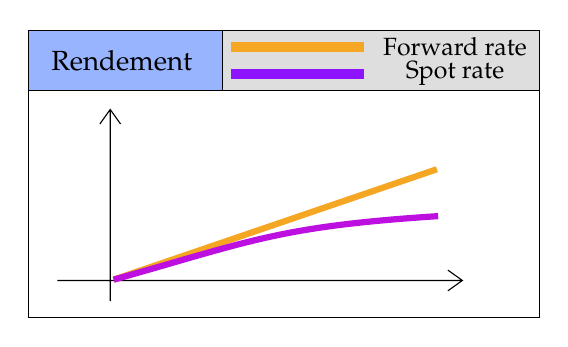
\begin{tikzpicture}[x=0.75pt,y=0.75pt,yscale=-1,xscale=1]
%uncomment if require: \path (0,300); %set diagram left start at 0, and has height of 300

%Shape: Rectangle [id:dp11598225207048363] 
\draw  [fill={rgb, 255:red, 255; green, 255; blue, 255 }  ,fill opacity=1 ] (48,51.33) -- (294.17,51.33) -- (294.17,189.72) -- (48,189.72) -- cycle ;
%Shape: Axis 2D [id:dp3788668579196355] 
\draw  (62,171.72) -- (257.17,171.72)(87.5,89.33) -- (87.5,181.72) (250.17,166.72) -- (257.17,171.72) -- (250.17,176.72) (82.5,96.33) -- (87.5,89.33) -- (92.5,96.33)  ;
%Straight Lines [id:da9101312021066204] 
\draw [color={rgb, 255:red, 245; green, 166; blue, 35 }  ,draw opacity=1 ][line width=2.25]    (89.17,171.33) -- (244.9,118.13) ;
%Shape: Rectangle [id:dp7987614739910429] 
\draw  [fill={rgb, 255:red, 152; green, 180; blue, 255 }  ,fill opacity=1 ] (48,51.33) -- (294.17,51.33) -- (294.17,80.13) -- (48,80.13) -- cycle ;
%Shape: Rectangle [id:dp9676581606760322] 
\draw  [fill={rgb, 255:red, 222; green, 222; blue, 222 }  ,fill opacity=1 ] (141.5,51.21) -- (294.17,51.21) -- (294.17,80.24) -- (141.5,80.24) -- cycle ;
%Straight Lines [id:da5630202320242259] 
\draw [color={rgb, 255:red, 142; green, 19; blue, 254 }  ,draw opacity=1 ][line width=3.75]    (145.6,72.33) -- (209.55,72.33) ;
%Straight Lines [id:da8305691123140908] 
\draw [color={rgb, 255:red, 245; green, 166; blue, 35 }  ,draw opacity=1 ][line width=3.75]    (145.6,59.13) -- (209.55,59.13) ;

%Curve Lines [id:da09193472671814629] 
\draw [color={rgb, 255:red, 189; green, 16; blue, 224 }  ,draw opacity=1 ][line width=2.25]    (89.17,171.33) .. controls (155.5,152.72) and (168.5,145.72) .. (245.5,140.72) ;

% Text Node
\draw (93.08,65.73) node   [align=left] {Rendement};
% Text Node
\draw (253.66,72.03) node  [font=\small] [align=left] {Spot rate};
% Text Node
\draw (253.66,58.84) node  [font=\small] [align=left] {Forward rate};


\end{tikzpicture}

\end{center}
\end{distributions}

\begin{algo}{Application aux obligations}
\begin{enumerate}[leftmargin = *]
	\item	Identifier les flux monétaires de l'obligation $CF_{t}$.
	\item	Actualiser chaque $CF_{t}$ selon son taux à terme $r_{t}$ pour déterminer le prix $P$.
	\item	Déterminer le taux de rendement $i$ (\og \textit{Yield-to-Maturity} \fg{} , \og \textit{IRR} \fg{}) qui, en actualisant les $CF_{t}$, reproduit le prix $P$.
	\item	$P = \underset{t}{\sum}\frac{CF_{t}}{(1 + r_{t})^{t}} = \underset{t}{\sum}\frac{CF_{t}}{(1 + i)^{t}}$
\end{enumerate}
\end{algo}

\newpage

\section{Analyse probabiliste des risques actuariels}
\subsection{Analyse combinatoire}
\begin{description}
	\item[Analyse combinatoire]	La théorie mathématique du comptage.
\end{description}

\begin{definitionNOHFILLsub}[Principe de base de comptage]
Deux expériences sont effectuées.	\\
La première a $m$ événements possibles, et la deuxième a $n$ événements possibles.	\\
Ensemble, il y a $m \times n$ événements possible pour les deux expériences.	

\tcbline

On peut visualiser ceci avec un tableau:
\begin{center}
\begin{tabular}{| >{\columncolor{beaublue}}c | >{\columncolor{beaublue}}c  | >{\columncolor{beaublue}}c  | >{\columncolor{beaublue}}c  |}
\hline
$(1, 1)$	&	$(1, 2)$	&	$\dots$	&	$(1, n)$	\\\hline
$(2, 1)$	&	$(2, 2)$	&	$\dots$	&	$(2, n)$	\\\hline
$\vdots$	&	$\vdots$	&	$\ddots$	&	$\vdots$	\\\hline
$(m, 1)$	&	$(m, 2)$	&	$\dots$	&	$(m, n)$	\\\hline
\end{tabular}
\end{center}
\begin{itemize}
	\item	Par exemple, la première cellule à l'événement 1 pour l'expérience 1 et l'événement 2 pour l'expérience 2.
\end{itemize}
\end{definitionNOHFILLsub}


\columnbreak
\subsection*{Théorèmes probabilistes}

\textbf{Théorème du binôme}
\begin{align*}
	(x + y)^{n}
		&=	\sum_{k = 0}^{n} \binom{n}{k} x^{k} y^{n - k}, \; \forall n \in \mathds{N}	\\
\end{align*}

%\subsubsection*{Coefficient multinomial}
%
%\begin{align*}
%	\binom{n}{n_{1}, \dots, n_{r}}
%		&=	\frac{n!}{n_{1}!\dots n_{r}!}
%\end{align*}

\textbf{Théorème multinomial}
\begin{align*}
	(x_1 + \dots + x_r)^{n}
		&=	\sum_{\substack{(n_1, \dots, n_r): \\ n_1 + \dots + n_r = n}} \binom{n}{n_{1}, \dots, n_{r}} x_{1}^{n_{1}} \dots x_{r}^{n_{r}}	
\end{align*}

\begin{minipage}[ht]{0.5\linewidth}
\textbf{Relations factoriels}

\begin{equation*}
	\binom{n}{k}
		=	\binom{n}{n - k}		
\end{equation*}
\end{minipage}
\begin{minipage}[ht]{0.5\linewidth}
\textbf{Règle de Pascal}

\begin{equation*}
	\binom{n}{k} + \binom{n}{k + 1}
		=	\binom{n + 1}{k + 1}		
\end{equation*}
\end{minipage}
\

\textbf{Triangle de Pascal}

\begin{minipage}{0.4\linewidth}
\tikzset{every picture/.style={line width=0.75pt}} %set default line width to 0.75pt        

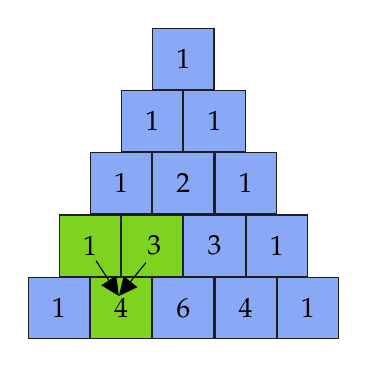
\begin{tikzpicture}[x=0.75pt,y=0.75pt,yscale=-1,xscale=1]
%uncomment if require: \path (0,300); %set diagram left start at 0, and has height of 300

%Shape: Square [id:dp6941490808398538] 
\draw  [color={rgb, 255:red, 31; green, 31; blue, 31 }  ,draw opacity=1 ][fill={rgb, 255:red, 137; green, 169; blue, 247 }  ,fill opacity=1 ] (192.5,0.33) -- (222,0.33) -- (222,29.83) -- (192.5,29.83) -- cycle ;

%Shape: Square [id:dp5483734211163716] 
\draw  [color={rgb, 255:red, 31; green, 31; blue, 31 }  ,draw opacity=1 ][fill={rgb, 255:red, 137; green, 169; blue, 247 }  ,fill opacity=1 ] (177.5,30.33) -- (207,30.33) -- (207,59.83) -- (177.5,59.83) -- cycle ;

%Shape: Square [id:dp6113568187175975] 
\draw  [color={rgb, 255:red, 31; green, 31; blue, 31 }  ,draw opacity=1 ][fill={rgb, 255:red, 137; green, 169; blue, 247 }  ,fill opacity=1 ] (207.5,30.33) -- (237,30.33) -- (237,59.83) -- (207.5,59.83) -- cycle ;

%Shape: Square [id:dp18321491615395535] 
\draw  [color={rgb, 255:red, 31; green, 31; blue, 31 }  ,draw opacity=1 ][fill={rgb, 255:red, 137; green, 169; blue, 247 }  ,fill opacity=1 ] (162.5,60.33) -- (192,60.33) -- (192,89.83) -- (162.5,89.83) -- cycle ;

%Shape: Square [id:dp5935951134760318] 
\draw  [color={rgb, 255:red, 31; green, 31; blue, 31 }  ,draw opacity=1 ][fill={rgb, 255:red, 137; green, 169; blue, 247 }  ,fill opacity=1 ] (192.5,60.33) -- (222,60.33) -- (222,89.83) -- (192.5,89.83) -- cycle ;
%Shape: Square [id:dp15135091580108684] 
\draw  [color={rgb, 255:red, 31; green, 31; blue, 31 }  ,draw opacity=1 ][fill={rgb, 255:red, 137; green, 169; blue, 247 }  ,fill opacity=1 ] (222.5,60.33) -- (252,60.33) -- (252,89.83) -- (222.5,89.83) -- cycle ;

%Shape: Square [id:dp6959691378679023] 
\draw  [color={rgb, 255:red, 31; green, 31; blue, 31 }  ,draw opacity=1 ][fill={rgb, 255:red, 126; green, 211; blue, 33 }  ,fill opacity=1 ] (147.5,90.33) -- (177,90.33) -- (177,119.83) -- (147.5,119.83) -- cycle ;

%Shape: Square [id:dp3401786459744438] 
\draw  [color={rgb, 255:red, 31; green, 31; blue, 31 }  ,draw opacity=1 ][fill={rgb, 255:red, 126; green, 211; blue, 33 }  ,fill opacity=1 ] (177.5,90.33) -- (207,90.33) -- (207,119.83) -- (177.5,119.83) -- cycle ;
%Shape: Square [id:dp054113641995666484] 
\draw  [color={rgb, 255:red, 31; green, 31; blue, 31 }  ,draw opacity=1 ][fill={rgb, 255:red, 137; green, 169; blue, 247 }  ,fill opacity=1 ] (207.5,90.33) -- (237,90.33) -- (237,119.83) -- (207.5,119.83) -- cycle ;
%Shape: Square [id:dp11590999892335718] 
\draw  [color={rgb, 255:red, 31; green, 31; blue, 31 }  ,draw opacity=1 ][fill={rgb, 255:red, 137; green, 169; blue, 247 }  ,fill opacity=1 ] (237.5,90.33) -- (267,90.33) -- (267,119.83) -- (237.5,119.83) -- cycle ;

%Shape: Square [id:dp23803207337642562] 
\draw  [color={rgb, 255:red, 31; green, 31; blue, 31 }  ,draw opacity=1 ][fill={rgb, 255:red, 137; green, 169; blue, 247 }  ,fill opacity=1 ] (132.5,120.33) -- (162,120.33) -- (162,149.83) -- (132.5,149.83) -- cycle ;

%Shape: Square [id:dp5531375567623269] 
\draw  [color={rgb, 255:red, 31; green, 31; blue, 31 }  ,draw opacity=1 ][fill={rgb, 255:red, 126; green, 211; blue, 33 }  ,fill opacity=1 ] (162.5,120.33) -- (192,120.33) -- (192,149.83) -- (162.5,149.83) -- cycle ;
%Shape: Square [id:dp4320593415188343] 
\draw  [color={rgb, 255:red, 31; green, 31; blue, 31 }  ,draw opacity=1 ][fill={rgb, 255:red, 137; green, 169; blue, 247 }  ,fill opacity=1 ] (192.5,120.33) -- (222,120.33) -- (222,149.83) -- (192.5,149.83) -- cycle ;
%Shape: Square [id:dp02227383517383874] 
\draw  [color={rgb, 255:red, 31; green, 31; blue, 31 }  ,draw opacity=1 ][fill={rgb, 255:red, 137; green, 169; blue, 247 }  ,fill opacity=1 ] (222.5,120.33) -- (252,120.33) -- (252,149.83) -- (222.5,149.83) -- cycle ;
%Shape: Square [id:dp7593605515111705] 
\draw  [color={rgb, 255:red, 31; green, 31; blue, 31 }  ,draw opacity=1 ][fill={rgb, 255:red, 137; green, 169; blue, 247 }  ,fill opacity=1 ] (252.5,120.33) -- (282,120.33) -- (282,149.83) -- (252.5,149.83) -- cycle ;

%Straight Lines [id:da6208300176170172] 
\draw [color={rgb, 255:red, 0; green, 0; blue, 0 }  ,draw opacity=1 ]   (165.17,112.33) -- (175.08,127.65) ;
\draw [shift={(176.17,129.33)}, rotate = 237.09] [fill={rgb, 255:red, 0; green, 0; blue, 0 }  ,fill opacity=1 ][line width=0.75]  [draw opacity=0] (8.93,-4.29) -- (0,0) -- (8.93,4.29) -- cycle    ;

%Straight Lines [id:da8782482964882432] 
\draw [color={rgb, 255:red, 0; green, 0; blue, 0 }  ,draw opacity=1 ]   (189.17,113.33) -- (177.43,127.78) ;
\draw [shift={(176.17,129.33)}, rotate = 309.09000000000003] [fill={rgb, 255:red, 0; green, 0; blue, 0 }  ,fill opacity=1 ][line width=0.75]  [draw opacity=0] (8.93,-4.29) -- (0,0) -- (8.93,4.29) -- cycle    ;


% Text Node
\draw (207.25,15.08) node  [align=left] {1};
% Text Node
\draw (192.25,45.08) node  [align=left] {1};
% Text Node
\draw (222.25,45.08) node  [align=left] {1};
% Text Node
\draw (207.25,75.08) node  [align=left] {2};
% Text Node
\draw (177.25,75.08) node  [align=left] {1};
% Text Node
\draw (237.25,75.08) node  [align=left] {1};
% Text Node
\draw (193.25,105.08) node  [align=left] {3};
% Text Node
\draw (162.25,105.08) node  [align=left] {1};
% Text Node
\draw (252.25,105.08) node  [align=left] {1};
% Text Node
\draw (222.25,105.08) node  [align=left] {3};
% Text Node
\draw (177.25,135.08) node  [align=left] {4};
% Text Node
\draw (207.25,135.08) node  [align=left] {6};
% Text Node
\draw (147.25,135.08) node  [align=left] {1};
% Text Node
\draw (267.25,135.08) node  [align=left] {1};
% Text Node
\draw (237.25,135.08) node  [align=left] {4};

\end{tikzpicture}
\end{minipage}
\begin{minipage}{0.6\linewidth}

\begin{itemize}
	\item	Triangle des coefficients binomiaux
	\item 	Chaque nombre est la somme des 2 nombres directement au-dessus.
\end{itemize}

\begin{align*}
	\binom{n}{k}
		&=	\binom{n - 1}{k - 1} + \binom{n - 1}{k}		\\
\end{align*}
\end{minipage}

\subsection*{Moments}

\begin{tabular}{| l | l |}
\hline
	Moment d'ordre $n$ \textit{(autour de l'origine)}.	&	$\text{E}[X^{n}] = \underset{i}{\sum} x_{i}^{n} \Pr(X = x_{i})$	\\
	Moment \textbf{\textit{centré}} d'ordre $n$.	&	$\text{E}[(X - \text{E}[X])^{n}] = \underset{i}{\sum} (x_{i} - \text{E}[X])^{n} \Pr(X = x_{i})$	\\
	Moment \textbf{\textit{réduit}} d'ordre $n$.&	$\text{E}\left[\left(\frac{X}{\sqrt{\text{V}(X)}}\right)^{n}\right] = \underset{i}{\sum} \left(\frac{x_{i}}{\sqrt{\text{V}(X)}}\right)^{n} \Pr(X = x_{i})$	\\
	Moment \textbf{\textit{centré-réduit}} d'ordre $n$.	&	$\text{E}\left[\left(\frac{X - \text{E}[X]}{\sqrt{\text{V}(X)}}\right)^{n}\right] = \underset{i}{\sum} \left(\frac{x_{i} - \text{E}[X]}{\sqrt{\text{V}(X)}}\right)^{n} \Pr(X = x_{i})$	\\
	Coefficient d'asymétrie \textit{(\textbf{Skewness})} 	&	$\gamma_{X} = \text{E}\left[\left(\frac{X - \text{E}[X]}{\sqrt{\text{V}(X)}}\right)^{3}\right]$	\\
	Coefficient d'aplatissement \textit{\textbf{(Kurtosis)}} 	&	$\kappa_{X} = \text{E}\left[\left(\frac{X - \text{E}[X]}{\sqrt{\text{V}(X)}}\right)^{4}\right]$	\\
	Fonction stop-loss 	&	$\pi_{X}(d) = \text{E}\left[\max(X - d; 0)\right]$	\\
	Fonction d'excès-moyen 	&	$\pi_{X}(d) = \text{E}\left[X - d | X > d\right]$	\\	\hline
\end{tabular}

\textbf{Note: } Il est intéressant de savoir que les moments impairs d'une loi normal avec moyenne nulle sont nuls.
Ceci est la normal avec une moyenne nulle est parfaitement symétrique tel que $f(-x) = -f(x)$; pour plus de détails, voir \href{https://www.youtube.com/watch?v=V4CjFT0k-_E}{ce vidéo YouTube}.

\begin{rappel}{Raccourci bernoulli}
Soit 
\begin{align*}
	X
	&=	\begin{cases}
		a	&	p	\\
		b	&	1 - p	\\
		\end{cases}
\end{align*}
Alors
\begin{align*}
	\text{Var}(X)	
	&=	(b - a)^{2}p (1 - p)
\end{align*}
\end{rappel}

\textbf{Conditionnels}
\begin{align*}
	\text{E}[X]	&=	\text{E}_{Y}[\text{E}[X|Y]]	&
	\text{V}(X)	&=	\text{E}_{Y}[\text{V}(X|Y)] + \text{V}_{Y}(\text{E}[X|Y])
\end{align*}

\begin{align*}
	\text{Cov}(X, Y)	
		&=	\text{E}[XY] - \text{E}[X] \text{E}[Y]	
\end{align*}

\begin{enumerate}
	\item $\text{Cov}(X, Y) = \text{Cov}(Y, X)$
	\item $\text{Cov}(X, X) = \text{V}(X)$
	\item $\text{Cov}(X, Y) \overset{\bot}{=} 0$
	\item $\text{Cov}(c, X) = 0$
	\item $\text{Cov}(cX, Y) = c\text{Cov}(X, Y)$
	\item $\text{Cov}(\sum_{i = 1}^{n}\alpha_{i} X_{i}, \sum_{j = 1}^{m}\beta_{j} Y_{j}) = \sum_{i = 1}^{n}\sum_{j = 1}^{m}\alpha_{i}\beta_{j}  \text{Cov}(X_{i}, Y_{j})$
\end{enumerate}

\begin{align*}
	\text{V}(\sum_{i = 1}^{n}\alpha_{i} X_{i}) 
		&= \sum_{i = 1}^{n}\sum_{j = 1}^{m}\alpha_{i}^{2}\text{V}(X_{i}) + 2 \underset{i < j}{\sum\sum} \alpha_{i}\alpha_{j} \text{Cov}(X_{i}, X_{j})	\\
	\rho_{\textrm{P}}(X, Y)
		&=	\frac{\text{Cov}(X, Y)}{\sigma_{X}\sigma_{Y}}
\end{align*}

\subsubsection*{Convolution}
\begin{definitionNOHFILLprop}[Convolution de deux variables aléatoires]
Soit deux v.a. continues indépendantes $X$ et $Y$.\\
Le produit de convolution de $X$ et $Y$ est :
\begin{align*}
	f_{X} \ast f_{Y}(s)
	=	f_{X + Y}(s)
	&=	\int_{-\infty}^{\infty}f_{X}(s - y)f_{Y}(y)dy	\\
	F_{X + Y}(s)
	&=	\int_{-\infty}^{\infty}F_{X}(s - y)f_{Y}(y)dy	\\
\end{align*}

\tcbline

Soit deux v.a. discrètes indépendantes $X$ et $Y$.\\
Le produit de convolution de $X$ et $Y$ est :
\begin{align*}
	\Pr(X + Y = s)
	&=	\sum_{y = 0}^{s}\Pr(X = s - y)\Pr(Y = y)	\\
\end{align*}

\end{definitionNOHFILLprop}

\subsection*{Variable aléatoire}

Soit X une variable aléatoire.

Soit la fonction

\begin{tabular}{| l | c | l |}
\hline
	de densité	&	$f_{X}(x) = \Pr(X = x)$	&	 Density Function	\\
	de masse de probabilité	&	$f_{X}(x) \neq \Pr(X = x)$	&	Probability Mass Function (PMF)	\\
	de répartition	&	$F_{X}(x) = \Pr(X \le x)$	&	Cumulative Density Function (CDF)\\
	de survie	&	$S_{X}(x) = \Pr(X > x)$	&	Survival Function (CDF)\\\hline	
\end{tabular}
$F_{X}(x)$

\subsection*{Lois multivariées}
	
\begin{rappel}{Loi multinomiale}
\begin{align*}
	\Pr(X_{1} = x_{1}, \dots, X_{r} = x_{r})
		&=	\binom{n}{x_{1}, \dots, x_{r}} p_{1}^{x_{1}} \dots p_{r}^{x_{r}}
\end{align*}
\end{rappel}

\begin{rappel}{Loi normale multivariée}
\begin{align*}
	f_{\matr{X}}(\matr{x}) 
		&= 	\frac{1}{(2 \pi)^{\frac{n}{2}} \sqrt{\text{det}(\bm{\Sigma})}} \e{\shortminus \frac{1}{2} (\matr{x} - \bm{\mu})^{\top} \bm{\Sigma}^{-1}(\bm{x} - \bm{\mu})}
\end{align*}
\end{rappel}

\columnbreak

\subsection*{Théorèmes limites}

\begin{algo}{Inégalité de Markov}
Soit la variable aléatoire (non-négative) $X$.\\
Alors $\forall a > 0$ on a:
\begin{align*}
	\Pr(X \ge a) 
	&\le 	\frac{\text{E}[X]}{a}
\end{align*}
\end{algo}

\begin{algo}{Inégalité de Tchebychev}
Soit la variable aléatoire $X$ avec $\mu, \sigma^{2} < \infty$.\\
Alors $\forall k > 0$ on a:
\begin{align*}
	\Pr\left( \left|X - \mu\right| \ge k \sigma\right)
	&\le 	\frac{1}{k^{2}}	&
	&\text{ou}	&
	\Pr\left( \left|X - \mu\right| \ge k^{*}\right)
	&\le 	\frac{\sigma^{2}}{(k^{*})^{2}}	\\
\end{align*}
\end{algo}

\begin{algo}{Loi (faible) des grands nombres (WLLN)}
Soit la suite de variables aléatoires (iid) $X_{1}, \dots, X_{n}$ tel que $\forall i = 1, \dots, n$ $\text{E}[X_{i}] = \mu$ et $\text{Var}[X_{i}] = \sigma^{2} > 0$.\\
Alors $\forall\epsilon > 0$ où $\bar{X}_{n} = \frac{X_{1} + \dots + X_{n}}{n}$:
\begin{align*} 
	\underset{n \rightarrow \infty}{\lim} \Pr\left( \left| \bar{X}_{n} -\mu \right| \ge \epsilon \right) 
	&\rightarrow		0	&
	&\Leftrightarrow	&
	\bar{X}_{n} \overset{\mathds{P}}{\underset{n \rightarrow \infty}{\longrightarrow}} \mu
\end{align*}
où $\mathds{P}$ représente la convergence en probablité.
\end{algo}

\begin{algo}{Théorème central limite (CLT)}
Soit la suite de variables aléatoires (iid) $X_{1}, \dots, X_{n}$ tel que $\forall i = 1, \dots, n$ $\text{E}[X_{i}] = \mu$ et $\text{Var}[X_{i}] = \sigma^{2} > 0$.\\
Alors pour $S_{n} = \sum_{i = 1}^{n} X_{i}$ :
\begin{align*} 
	\underset{n \rightarrow \infty}{\lim} \Pr\left( \frac{S_{n} - \text{E}[S_{n}]}{\sqrt{\text{Var}(S_{n})}} \le z \right) 
	&=	\Phi(z)
	&\Leftrightarrow	&
	\frac{S_{n} - \text{E}[S_{n}]}{\sqrt{\text{Var}(S_{n})}} \overset{\mathcal{L}}{\longrightarrow} \mathcal{N}(0, 1)
\end{align*}
où $\mathcal{L}$ représente la convergence en distribution ("law").
\end{algo}


\pagebreak
\section{Méthodes numériques}

\begin{center}
\begin{tabular}{| >{\columncolor{beaublue}}c | >{\columncolor{beaublue}}c  | >{\columncolor{beaublue}}c  |}
\hline\rowcolor{airforceblue} 
\textcolor{white}{\textbf{Unité}}	&	\textcolor{white}{\textbf{Capacité}}	&	\textcolor{white}{\textbf{Symbole}}		\\\hline
Bit	&	1 b	&	b	\\\hline
Octet (« \textit{byte} ») \fg{}	&	8 b	&	o	\\\hline
Kilooctet	&	1\ 024 o	&	ko	\\\hline
Megaoctet	&	1\ 048\ 576 o	&	mo	\\\hline
Gigaoctet	&	1\ 073\ 741\ 824 o	&	go	\\\hline
\end{tabular}
\end{center}

\end{multicols*}

\end{document}
